\sys is a new programming and execution model for intermittent computing on energy-harvesting devices. \sys addresses the challenges outlined in Section~\ref{sec:background} to make task-based intermittent programs {\em programmable} and {\em efficient}. \sys accomplishes this goal with a constellation of a new programming model and run time software system support, that supports dynamically adaptive task-based execution. Figure~\ref{fig:system_overview} shows an overview of \sys.

\textbf{\sys Programming and Execution Model.}  To use \sys, a programmer first writes plain, imperative C code. The programmer then must decompose the program into tasks. To manually decompose a program into tasks, the programmer designates a set of functions as tasks, sequences control-flow between these tasks, and annotates memory accesses that manipulate data shared by multiple tasks. In other words, it requires reasoning similar to prior task-based systems~\cite{chain,alpaca}. 

\begin{wrapfigure}{t!}{0.5\textwidth}
	\centering
	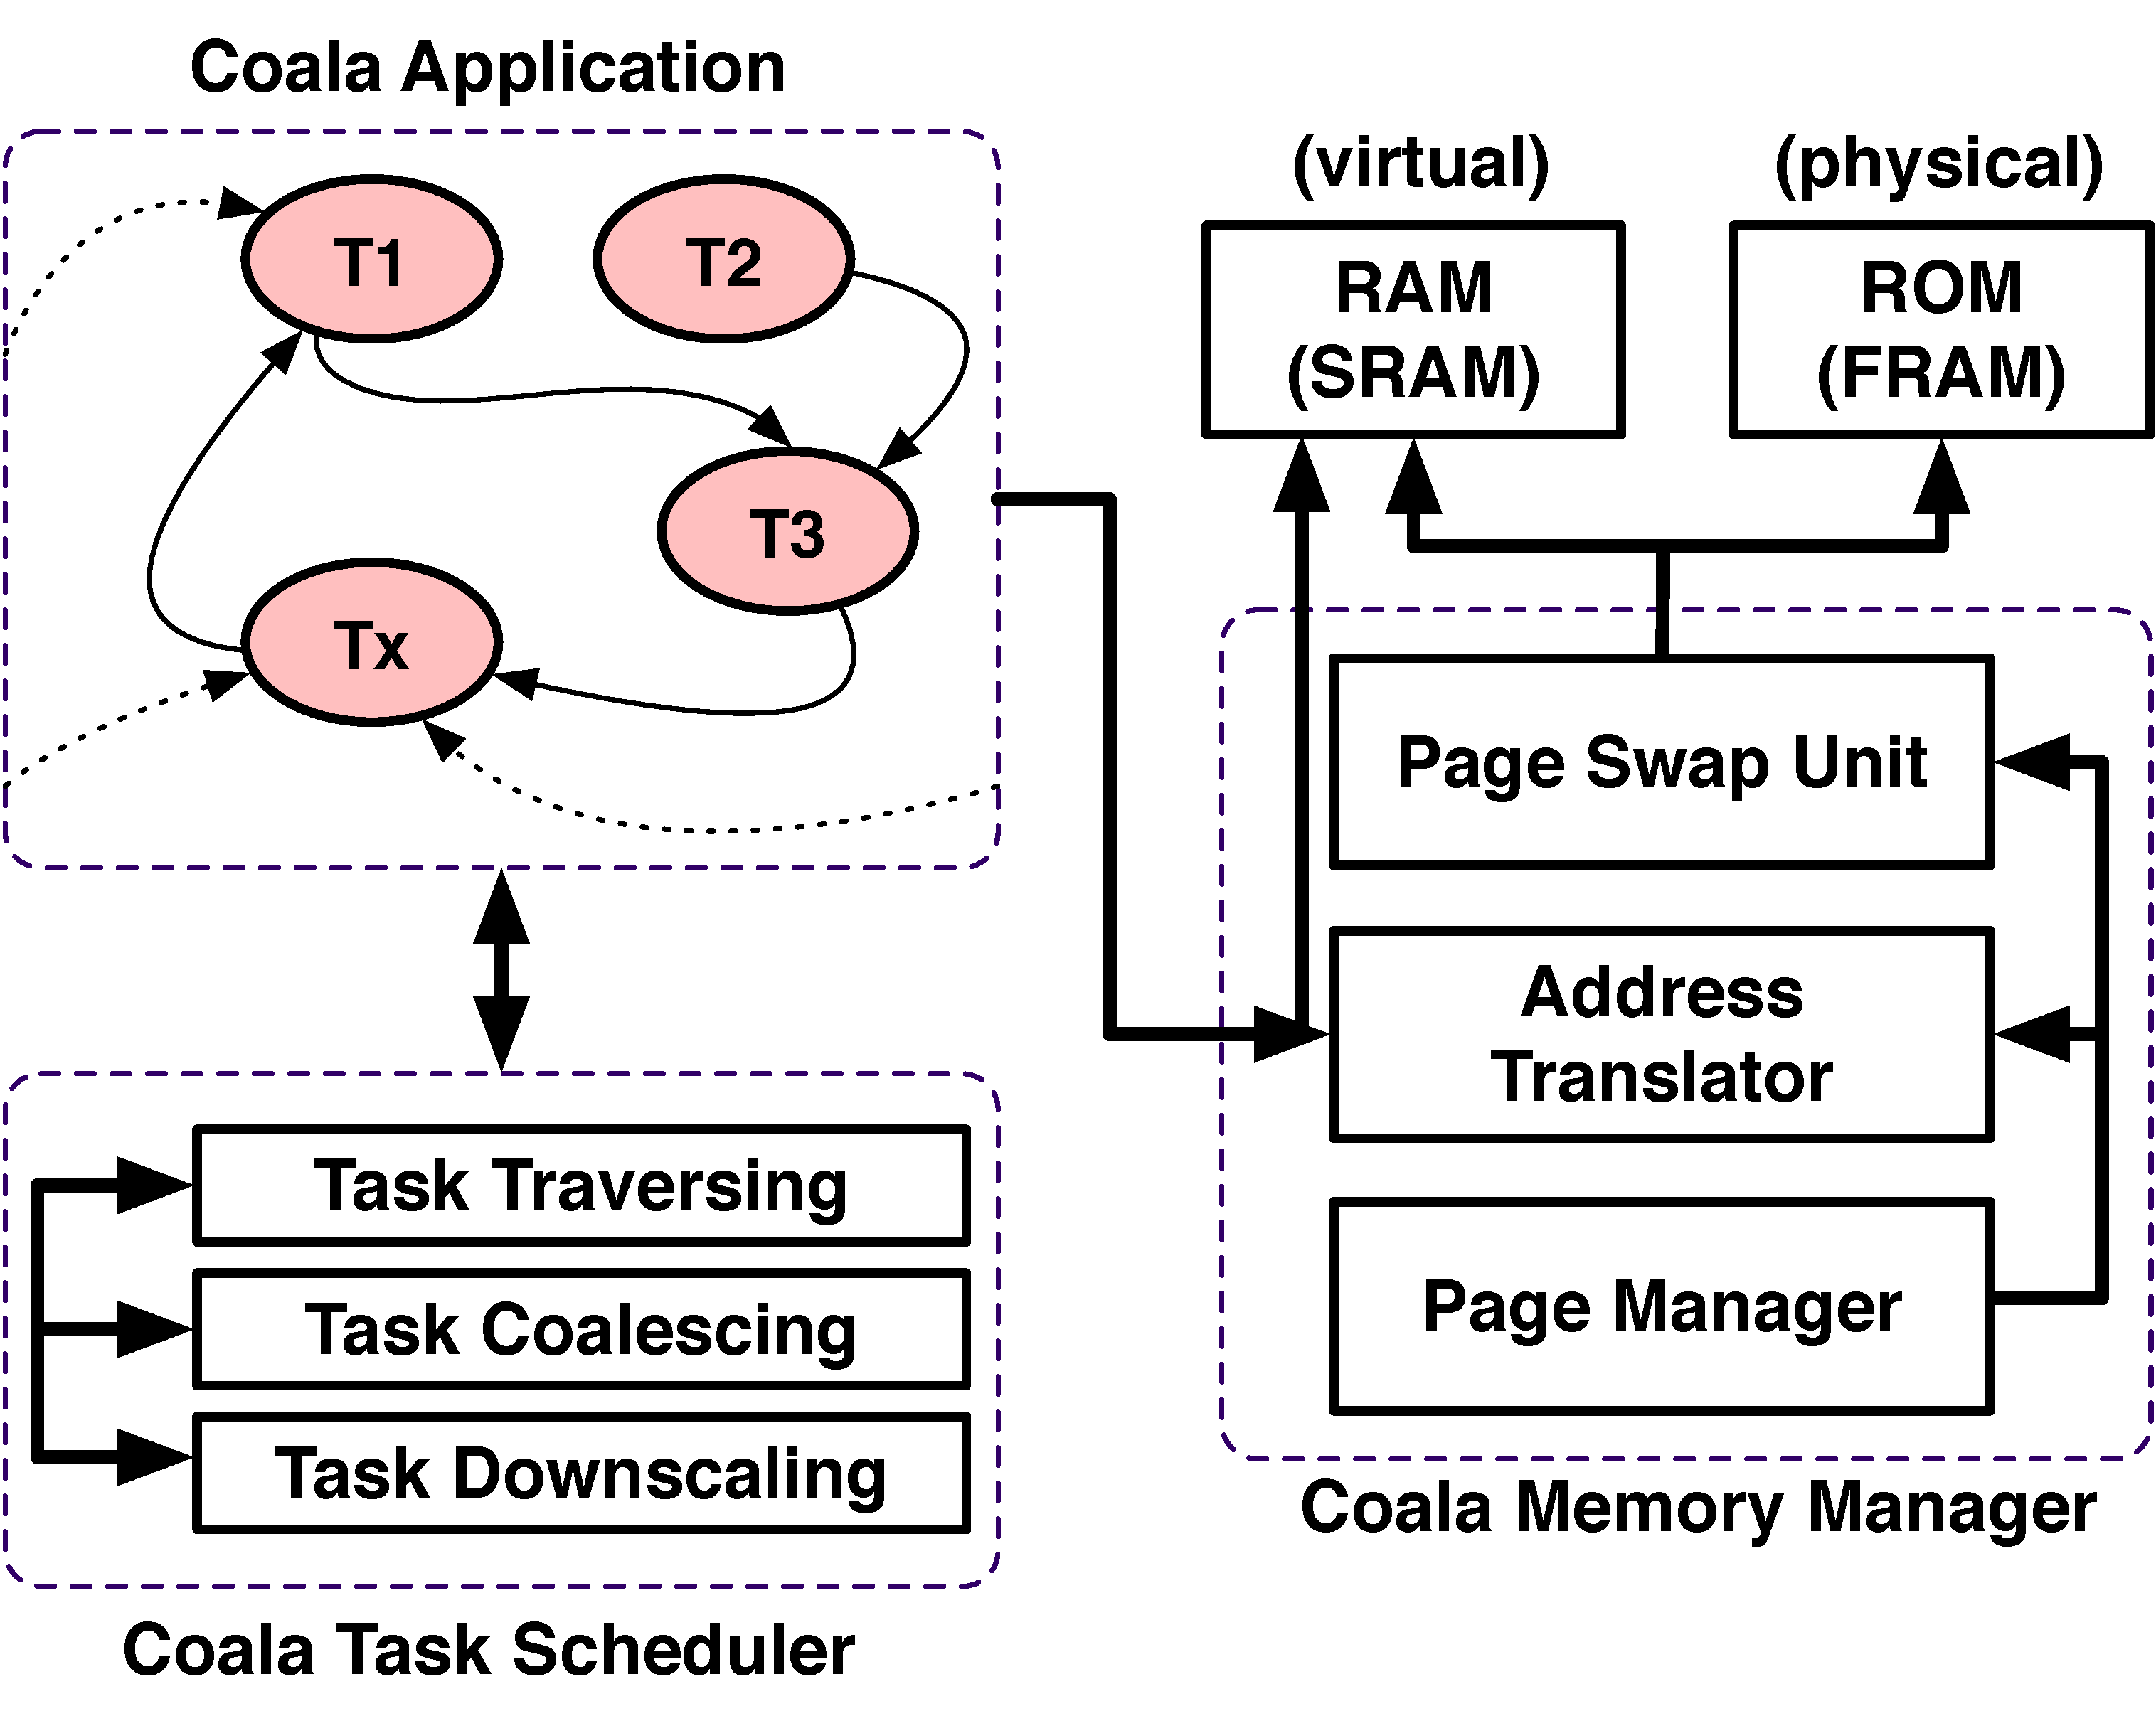
\includegraphics[width=0.5\columnwidth]{figures/graffle/overview.pdf}
	\caption{\sys top-level view. \sys is composed of two core components: \emph{Task Scheduler} and \emph{Memory Manager}.}
	\label{fig:system_overview}
\end{wrapfigure}

A programmer may also opt to use compiler support to automatically decompose a program into tasks, leveraging recent work~\cite{cleancut_2018,baghsorkhi_cgo_2018}. Without loss of generality, we assume throughout this work that the programmer manually decomposed the program into tasks; \sys's behavior with automatically decomposed code would be identical.

The programmer compiles their task-based code, and links to the \sys runtime, producing a \sys-enabled binary. The \sys runtime implements \sys's task-based programming and execution model. The runtime system also includes \sys's novel {\em virtualizing memory manager} and its {\em task coalescing manager}, and {\em task downscaling manager}, both of which are essential to \sys's adaptive task-based execution.

\textbf{\sys Task Coalescing Manager.} \sys relies on its task coalescing manager to dynamically {\em coalesce} statically\hyp{}defined tasks to avoid inessential overheads associated with completing tasks. By default, tasks run in a sequence and each task commits its task-shared state as it completes.  The time and energy cost of a task's commit is unnecessary if the task and its successor both complete without a power failure. The key insight that \sys leverages is that the first task could have deferred its commit to the second task. {\em coalescing} tasks by deferring the first commit avoids the fixed cost of the first commit (task transitioning overheads). Coalescing also amortizes per-variable commit cost, committing each location accessed by both tasks only after the second task, rather than once per task. \textcolor{red}{\sys's coalescing manager is an \emph{energy-aware manager}. It uses the recent execution history---pure software technique---as a metric to estimate the amount of the available energy and to set the adequate coalesced task size accordingly. This fundamental feature prevents \sys from blind coalesced task adaptation which may result in a repeated power failure problem. For example, If \sys enlarges the coalesced task size by $x$ static tasks on a coalesced task completion and reduces it by the same number of static tasks on a power reboot, then \sys may need to reboot, for instance, 10 times to reduce a coalesced task size from 10 to one, when $x=1$}. Details of coalescing are presented in Section~\ref{sec:task_coalescing}.

\textbf{\sys Task Downscaling Manager.} \textcolor{red}{\sys's downscaling manager is responsible for preserving the forward progress when \sys repeatedly fails on a single static task. The downscaling manager utilizes a timer-based technique and relies on the virtual memory manager to gain a full \emph{flexibility} on where to split a task. These features distinguish \sys task splitting technique from the traditional checkpointing. A checkpointing system that uses voltage threshold to place a checkpoint might cause a program to crash if the checkpoint happened to be placed between a peripheral initialization and its call. If a programmer disables interrupts between the peripheral initialization and the call, the program may fail indefinitely to progress since the checkpoint may only be deferred. The \sys task downscaling manager, on the other hand,  triggers  a \emph{partial commit} faster than the previous one on a repeated failure to guarantee forward progress. Details of task downscaling are presented in Section~\ref{sec:task_downsizing}.} 


\textbf{\sys Virtual Memory Manager.} \sys is able to efficiently coalesce tasks because of its efficient virtual memory manager, which is described in Section~\ref{sec:memory_virtualization}. \sys's memory manager paginates memory and ensures that data in a page remain consistent despite power interruptions. \sys allows a task to manipulate data in a volatile copy of a page only. Pages swap between volatile and non-volatile memory, depending on the capacity of the volatile memory and the program's access pattern. \sys tracks a task's memory accesses efficiently at page granularity (rather than using, e.g., costly word-granular tracking). When a task ends, each page it accessed commits from volatile memory (or from a non-volatile swap region for dirty pages) back to the non-volatile main memory. Pages efficiently, atomically commit using a two-phase commit procedure accelerated using hardware support for direct memory access (DMA). Details of Virtual Memory Manager are presented in Section~\ref{sec:memory_virtulaization}.